\documentclass{beamer}

\usepackage{beamerthemesplit}
\usepackage{verbatim}
\usepackage[normalem]{ulem}

\usepackage{xcolor}

\usepackage{hyperref}

\definecolor{gold}{rgb}{1.,0.84,0.}
\definecolor{brightred}{rgb}{1.,0.4,0.4}
\definecolor{mygray}{RGB}{200,200,200}
\definecolor{lightsteelblue}{RGB}{176,196,222}
\definecolor{lightskyblue}{RGB}{135,206,250}
\definecolor{cadetblue}{RGB}{95,158,160}

\usetheme{default}
\usecolortheme{mule}

\usefonttheme{serif}

%\DeclareGraphicsExtensions{.pdf,.png,.jpg}

\newcommand{\mcal}{\textsc{metacalibration}}
\newcommand{\Mcal}{\textsc{Metacalibration}}

\newcommand{\mcalR}{\mbox{\boldmath $R$}}
\newcommand{\mcalRscalar}{\mbox{$R$}}

\newcommand{\mcalRmean}{\mbox{\boldmath $\langle R \rangle$}}
\newcommand{\mcalRscalarmean}{\mbox{$\langle R \rangle$}}

\newcommand{\mcalRpsf}{$R^{p}$}
\newcommand{\mcalRpsfnoise}{$R^{p}_\eta$}
\newcommand{\mcalRo}{\mbox{\boldmath $R_o$}}
\newcommand{\mcalRnoise}{\mbox{\boldmath $R_\eta$}}

\newcommand{\mcalRmeanalpha}{\mbox{\boldmath $\langle R_\alpha \rangle$}}
\newcommand{\mcalRmeanbeta}{\mbox{\boldmath $\langle R_\beta \rangle$}}

\newcommand{\mcalRg}{\mbox{\boldmath $R_\gamma$}}
\newcommand{\mcalRS}{\mbox{\boldmath $R_S$}}
\newcommand{\mcalRgmean}{\mbox{\boldmath $\langle R_\gamma \rangle$}}
\newcommand{\mcalRSmean}{\mbox{\boldmath $\langle R_S \rangle$}}

\newcommand{\mcalRtwopt}{\mbox{\boldmath $R^{2pt}$}}
\newcommand{\mcalRtwoptmean}{\mbox{\boldmath $\langle R^{2pt} \rangle$}}


\newcommand{\mcalRmodel}{\mbox{\boldmath $R^{model}$}}
\newcommand{\mcalRnoisemodel}{\mbox{\boldmath $R^{model}_\eta$}}


\newcommand{\vecg}{\mbox{\boldmath $\gamma$}}
\newcommand{\vest}{\mbox{\boldmath $e$}}

\newcommand{\snr}{$S/N$}
\newcommand{\snT}{$(S/N)_{\textrm{size}}$}
%\newcommand{\snT}{$\left( \frac{S}{N}\right)_{\textrm{size}}$}
\newcommand{\snflux}{$(S/N)_{\textrm{flux}}$}
%\newcommand{\snflux}{$\left( \frac{S}{N}\right)_{\textrm{flux}}$}

\newcommand{\lensfit}{\texttt{LENSFIT}}
\newcommand{\numba}{\texttt{Numba}}
\newcommand{\python}{\texttt{Python}}
\newcommand{\ngmix}{\texttt{ngmix}}
\newcommand{\shear}{{\bf g}}
\newcommand{\redmapper}{redMaPPer}
\newcommand{\est}{$e$}


\newcommand{\prelim}{{\bf{\it Preliminary}}}

\newcommand{\uberseg}{{\"u}berseg}


\title{\Mcal\ Overview}
\author{Erin Sheldon}
\institute{Brookhaven National Laboratory}

% http://texblog.net/latex-archive/plaintex/beamer-footline-frame-number/
% to add the page (frame ) number and not screw up the bottom line
% works for split themes?
\expandafter\def\expandafter\insertshorttitle\expandafter{%
      \insertshorttitle\hfill%
        \insertframenumber\,/\,\inserttotalframenumber}

% suppress navigation bar
\beamertemplatenavigationsymbolsempty
\setbeamertemplate{footline}{}

\begin{document}

\usebackgroundtemplate{%
    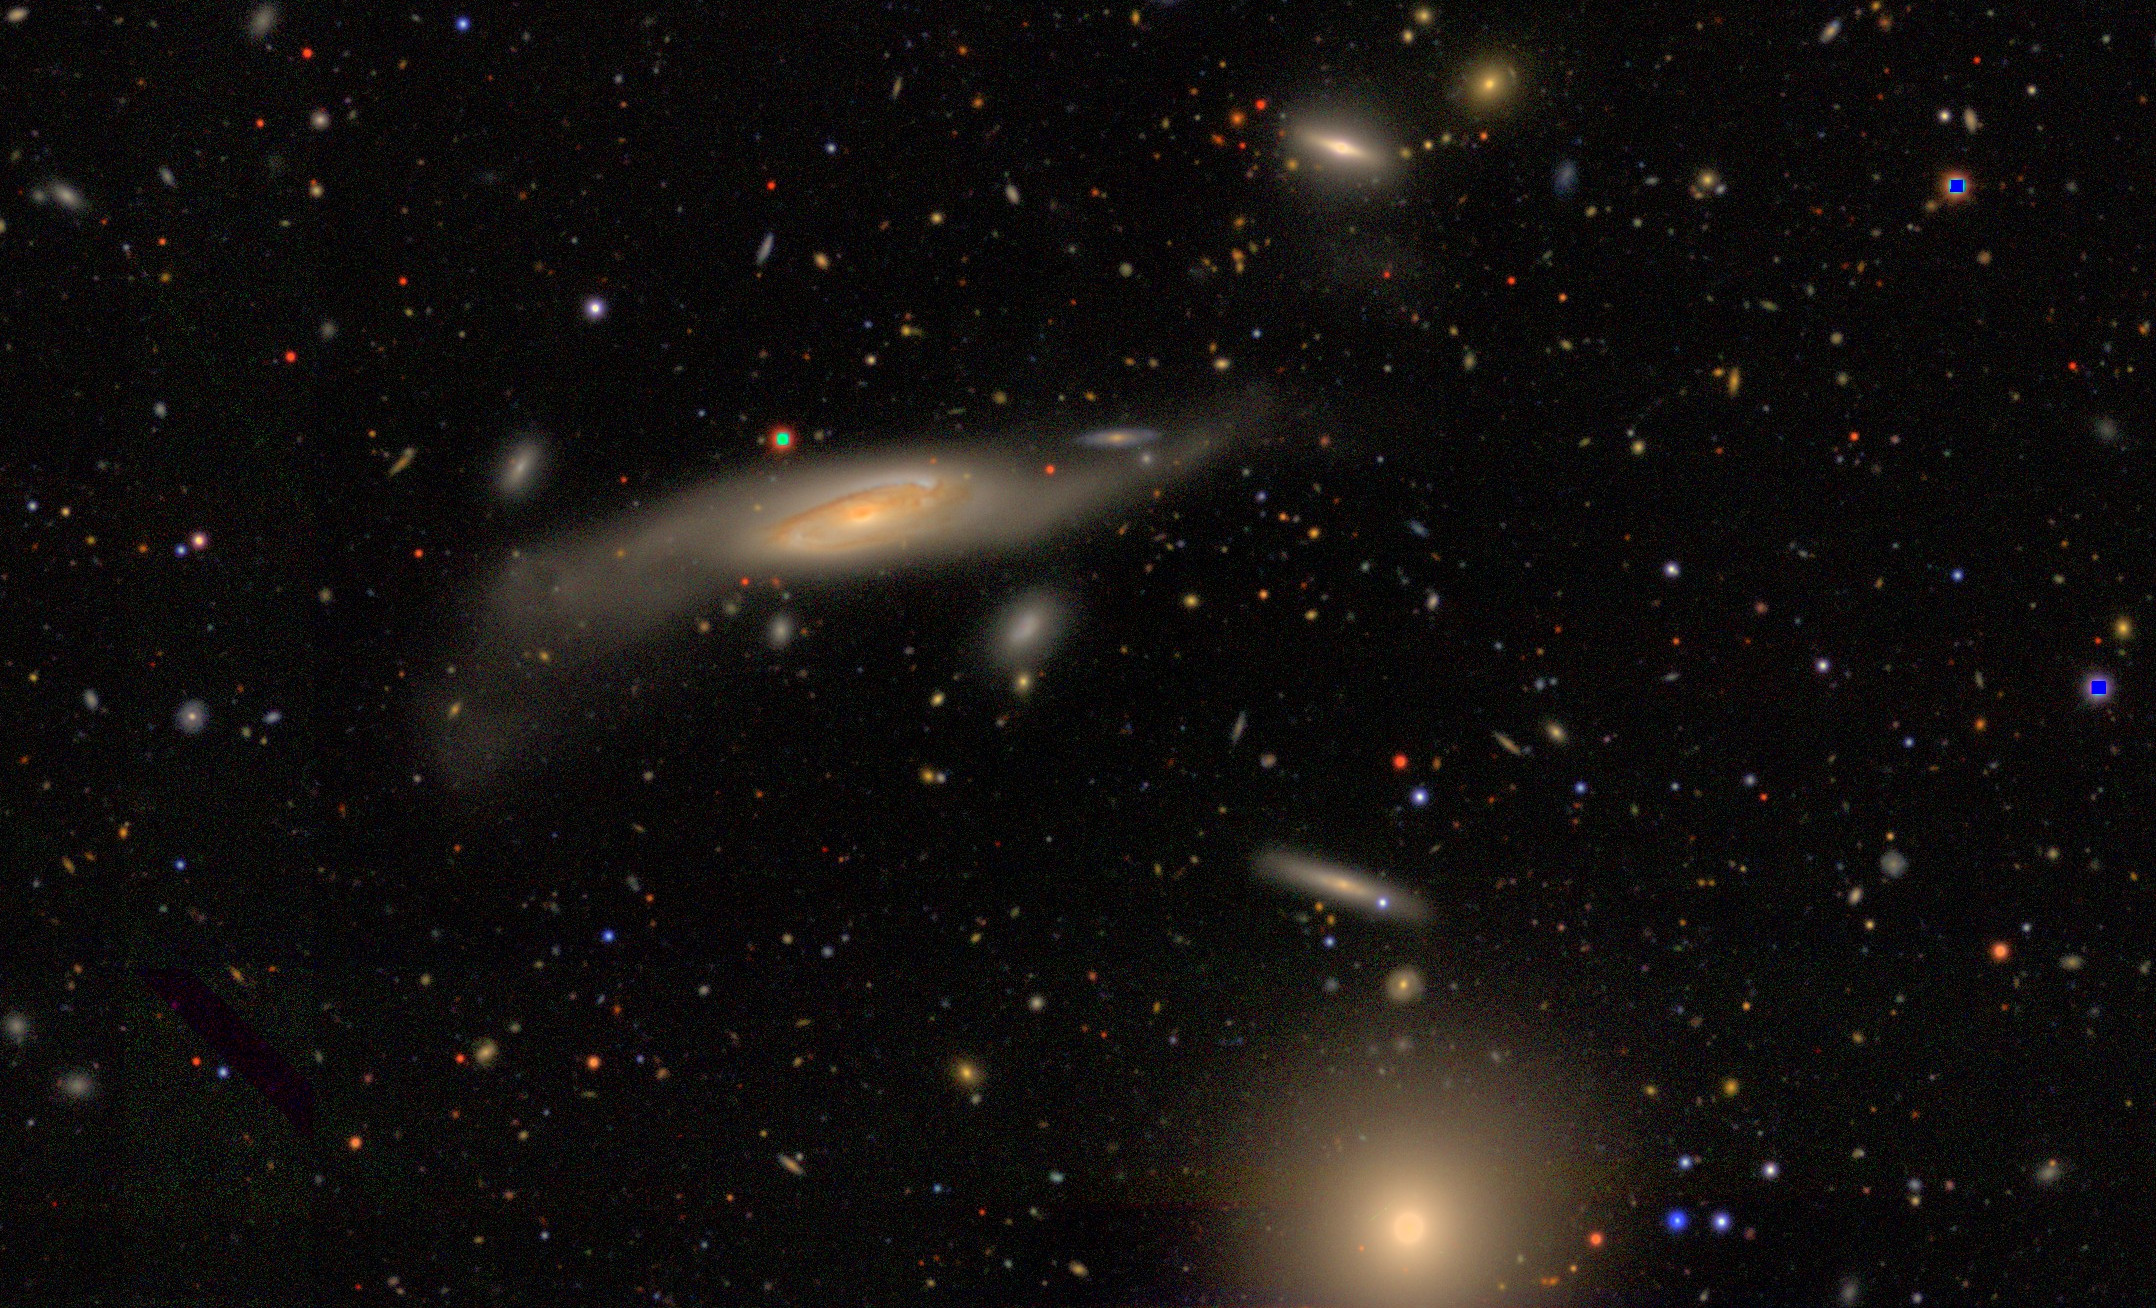
\includegraphics[height=\paperheight]{DES0056-5248_gri_crop.jpg}}
\frame
{
}
\setbeamertemplate{background canvas}[vertical shading][bottom=mgray,top=mblack]



\frame{\titlepage}

\setbeamerfont*{itemize/enumerate body}{size=\Large}
\setbeamerfont*{itemize/enumerate subbody}{parent=itemize/enumerate body}
\setbeamerfont*{itemize/enumerate subsubbody}{parent=itemize/enumerate body}



\frame
{
    \frametitle{Outline}

    \setbeamerfont*{itemize/enumerate body}{size=\Large}
    \setbeamerfont*{itemize/enumerate subbody}{parent=itemize/enumerate body}
    \setbeamerfont*{itemize/enumerate subsubbody}{parent=itemize/enumerate body}
 
    \begin{itemize}

        \item Introduction to \mcal
        \item Catalogs
        \item How to use the catalogs

    \end{itemize}

}


\frame
{
    \frametitle{\Mcal}

    \setbeamerfont*{itemize/enumerate body}{size=\Large}
    \setbeamerfont*{itemize/enumerate subbody}{parent=itemize/enumerate body}
    \setbeamerfont*{itemize/enumerate subsubbody}{parent=itemize/enumerate body}
 
 \begin{itemize}
     \item Designed to correct for noise bias, model bias, selection bias.
     \item No reliance on simulations or significant prior information
         for basic shear calibration.
 \end{itemize}

}

\frame
{
    \frametitle{\Mcal\ Idea from Eric Huff (Kaiser)}

    \setbeamerfont*{itemize/enumerate body}{size=\large}
    \setbeamerfont*{itemize/enumerate subbody}{parent=itemize/enumerate body}
    \setbeamerfont*{itemize/enumerate subsubbody}{parent=itemize/enumerate body}
 
    \begin{itemize}

        \item Suppose we have a biased shear estimator {\color{gold} \vest}.  Then we can write
            {\color{gold}
\begin{align} \label{eq:Eexpand}
    \vest &= \vest|_{\gamma=0} + \frac{ \partial \vest }{ \partial \vecg}\bigg|_{\gamma=0} \vecg  + ... \nonumber \\
          &\equiv \vest|_{\gamma=0} + \mbox{\mcalR}\vecg  + ...
\end{align}
            } 

        \item For an ensemble mean
            {\color{gold}
                \begin{align}
                    \langle \vest \rangle &= \langle \vest \rangle |_{\gamma=0} + \langle \mbox{\mcalR} \vecg \rangle + ... \nonumber \\
                                          &\approx \langle \mbox{\mcalR} \vecg \rangle,
                \end{align}
                }

            \item The shear is weighted by responses {\color{cadetblue} \mcalR}.  If we know the
                responses, we can form a weighted average:
            {\color{gold}
\begin{align} \label{eq:rcorr}
    \langle \vecg \rangle &\approx \langle \mbox{\mcalR} \rangle^{-1}  \langle \vest \rangle \approx \langle \mbox{\mcalR} \rangle^{-1} \langle \mcalR \vecg \rangle.
\end{align}
            }
    \end{itemize}
}

\frame
{
    \setbeamerfont*{itemize/enumerate body}{size=\Large}
    \setbeamerfont*{itemize/enumerate subbody}{parent=itemize/enumerate body}
    \setbeamerfont*{itemize/enumerate subsubbody}{parent=itemize/enumerate body}
 
    \frametitle{Numerical Derivative}

       \begin{itemize}

        \item Use image manipulation to estimate the derivative of the
            estimator with respect to shear
            {\color{gold}
                \begin{equation}
                    \mcalR = \frac{\vest^+ - \vest^-}{\Delta \vecg} \nonumber 
                \end{equation}
            }
            \begin{itemize}
                \item Deconvolve the PSF
                \item Shear the image by a small amount
                \item Reconvolve by a new function.  Should be larger than PSF to suppress
                    noise amplification. 
                \item {\color{lightsteelblue} Add noise field to cancel correlated noise}
            \end{itemize}


    \end{itemize}

}


\frame
{
    \frametitle{Selection Effects}

    \setbeamerfont*{itemize/enumerate body}{size=\Large}
    \setbeamerfont*{itemize/enumerate subbody}{parent=itemize/enumerate body}
    \setbeamerfont*{itemize/enumerate subsubbody}{parent=itemize/enumerate body}
 

    \begin{itemize}

        \item  Applying a selection to objects can indirectly select on the shapes
            of galaxies and result in a biased shear measurement.

        \item For example, putting a threshold on \snr\ tends to select less
            elliptical galaxies.

        \item Cannot be ignored: this is a percent level effect.

    \end{itemize}

}

\frame
{
    \frametitle{Selection Effects}

    \setbeamerfont*{itemize/enumerate body}{size=\large}
    \setbeamerfont*{itemize/enumerate subbody}{parent=itemize/enumerate body}
    \setbeamerfont*{itemize/enumerate subsubbody}{parent=itemize/enumerate body}
 
    \begin{itemize}

        \item If we have a selection function $S$ that has some dependence
            on ellipticity, then the mean ellipticity
            can be biased

            \begin{align}
                {\color{gold} \langle \vest \rangle^S = \int S(\vest)~P(\vest)~\vest~d\vest},
            \end{align}


        \item We can also use quantities measured from sheared images
            to correct for selections. 

            \begin{align}
                \frac{\partial \langle \vest \rangle}{\partial \gamma}\bigg|_{\gamma=0} &\approx
                \frac{\langle \vest^+ \rangle^S - \langle \vest^- \rangle^S}{\Delta \gamma} + \frac{\langle \vest \rangle^{S+} - \langle \vest \rangle^{S-}}{\Delta \gamma} \nonumber \\
                &\equiv {\color{gold} \langle \mcalRg \rangle + \langle \mcalRS \rangle},
            \end{align}

            Where {\color{lightsteelblue} $\langle \vest \rangle^{S+}$}
            represents the mean shape from unsheared images, with selection
            based on parameters measured from
            positively sheared images.

    \end{itemize}


}

\frame
{

 
    \frametitle{Two Recent Papers on \mcal}

    \begin{itemize}

        \item Huff \& Mandelbaum 2017: showed \mcal\ can calibrate even very
            noisy estimators on the GREAT3 sims (moderately challenging).

        \item Sheldon \& Huff 2017: tests on very challenging sims,
            including selection effects, using a less noisy estimator,
            no bias found.


    \end{itemize}

}

\frame
{


    \frametitle{Tests on Y1 Data}

    \begin{itemize}

        \item There are a slew of tests in the Y1 shear catalog paper (Zuntz,
            give link)

        \item The most important biases are caused by inaccurate PSF modeling
            and the blending of the light of neighboring objects.


        %\item PSF errors cause important additive biases that can
        %    strongly effect the shear 2pt function.  We are correcting
        %    for this in measurement itself (N. MacCrann).  We
        %    find the multiplicative bias from the PSF model errors to
        %    be relatively small.

        \begin{center}
            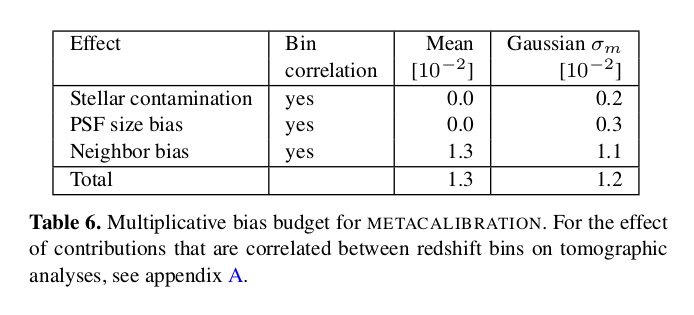
\includegraphics[width=0.8\textwidth]{mcal-bias.png}
            \newline
        \end{center}


    \end{itemize}

}


\frame
{
    \frametitle{Catalogs}

    \begin{itemize}
        \item Blinded catalogs are available (blinded coming soon)

        \item \url{https://cdcvs.fnal.gov/redmine/projects/deswlwg/wiki/Matched_catalogs}


    \end{itemize}
}

\frame
{
    \frametitle{How to Use the Catalogs}

    \setbeamerfont*{itemize/enumerate body}{size=\large}
    \setbeamerfont*{itemize/enumerate subbody}{parent=itemize/enumerate body}
    \setbeamerfont*{itemize/enumerate subsubbody}{parent=itemize/enumerate body}
 
    \begin{itemize}

        \item How to use the catalogs depends on the statistic you are measuring
            (Sheldon \& Huff 2017).

        \item In DES Y1 we have found that the mean response depends weakly on
            separation between galaxies over the scales of interest, so one
            need only calculate the mean response for ggl and shear 2-pt
            functions.

        \item If you are calculating a statistic other than mean shear or
            2-pt shear, let's discuss how to calculate responses.  It may
            require a specially crafted calibration.

        \item See papers for examples (mass mapping, shear 2pt, etc.) as well
            as the DES wiki
            \url{https://cdcvs.fnal.gov/redmine/projects/deswlwg/wiki/MetacalibrationUsingCatalogs}

    \end{itemize}
}


\frame
{
    \frametitle{How to Use the Catalogs: Mass Mapping}

    \setbeamerfont*{itemize/enumerate body}{size=\large}
    \setbeamerfont*{itemize/enumerate subbody}{parent=itemize/enumerate body}
    \setbeamerfont*{itemize/enumerate subsubbody}{parent=itemize/enumerate body}
 
    \begin{itemize}

        \item Some mass mapping statistics start with just the mean
            shear in bins.  This is the example we worked out above

            \begin{align}
                \frac{\partial \langle \vest \rangle}{\partial \gamma}\bigg|_{\gamma=0} &\approx
                \frac{\langle \vest^+ \rangle^S - \langle \vest^- \rangle^S}{\Delta \gamma} + \frac{\langle \vest \rangle^{S+} - \langle \vest \rangle^{S-}}{\Delta \gamma} \nonumber \\
                &\equiv {\color{gold} \langle \mcalRg \rangle + \langle \mcalRS \rangle = \mcalR},
            \end{align}

            {\color{gold}
\begin{align} \label{eq:rcorr}
    \langle \vecg \rangle &\approx \langle \mbox{\mcalR} \rangle^{-1}  \langle \vest \rangle \approx \langle \mbox{\mcalR} \rangle^{-1} \langle \mcalR \vecg \rangle
\end{align}
            }

        \item {\color{gold} \mcalRgmean} is typically 0.6 
        \item {\color{gold} \mcalRSmean} is typically 0.01

        \item Cannot ignore selection effects, would get the shear calibration
            wrong by 2\%.


    \end{itemize}
}

\frame
{
    \frametitle{How to Use the Catalogs: 2-pt shear}

    \setbeamerfont*{itemize/enumerate body}{size=\large}
    \setbeamerfont*{itemize/enumerate subbody}{parent=itemize/enumerate body}
    \setbeamerfont*{itemize/enumerate subsubbody}{parent=itemize/enumerate body}
 
    \begin{itemize}

        \item The response appears to be independent of galaxy separation over
            the relevant scales, basically just need to divide by {\color{gold}
            \mcalRmean$^2$}

        \item {\color{gold} \mcalRgmean} is typically 0.6 
        \item {\color{gold} \mcalRSmean} is typically 0.01 to 0.02

        \item Cannot ignore selection effects, would get the shear calibration
            wrong by 2-4\%.


    \end{itemize}
}




\frame
{
    \frametitle{How to Use the Catalogs: Averaging Related Quantities}
 
    \begin{itemize}

        \item If you average a related quantity, such as redshift, $P(z)$,
            etc. you should apply the shear responses as weights

            {\color{gold}
                \begin{align}
                    \langle x \rangle = \frac{\sum \mcalRg x}{\sum \mcalRg}
                \end{align}
            }

        \item We have been averaging the diagonal elements of the
            response matrix

            {\color{gold}
                \begin{align}
                    0.5 \times ( \mcalRg[0,0] + \mcalRg[1,1] )
                \end{align}
            }
    \end{itemize}
}







\frame
{
    \frametitle{Extra Slides}
}


\frame
{
    \frametitle{Sources of Systematic Error in Typical Estimators}

    \setbeamerfont*{itemize/enumerate body}{size=\large}
    \setbeamerfont*{itemize/enumerate subbody}{parent=itemize/enumerate body}
    \setbeamerfont*{itemize/enumerate subsubbody}{parent=itemize/enumerate body}
 
    \begin{itemize}

        \item Galaxy models used to infer ellipticity and shear 
            typically wildly inaccurate, error exceeds budget.

        \item Noise biases shape determination, error exceed budget.

        \item Most of the galaxies in ground based surveys are
            poorly resolved, worsening modeling and noise effects.

        \item Selection effects can easily exceed error budget.

        \item Effects of neighbors and undetected objects can cause
            large bias, especially when calibrating from simulations.

        \item PSF Modeling must be accurate (effects {\em all} known estimators)

    \end{itemize}

}


\frame
{
    \frametitle{Correlated Noise}

    \setbeamerfont*{itemize/enumerate body}{size=\large}
    \setbeamerfont*{itemize/enumerate subbody}{parent=itemize/enumerate body}
    \setbeamerfont*{itemize/enumerate subsubbody}{parent=itemize/enumerate body}
 

    \begin{itemize}

        \item Convolutions and shearing result in correlated noise.

        \item At \snr$\sim 10$ can cause a 10\% shear bias.

        \item Add a noise field that has been run through the same
            operations, and then rotated by 90 degrees.

        \item Cancels all correlated noise effects
            
            \begin{itemize}
                \item Increases the noise in the shear recovery by 20\% (less
                    than $\sqrt 2$ because shape noise dominates).

                \item Even smaller relative effect
                    for cosmic shear which is sample variance dominated
                \item Search for a less noisy correction is ongoing
             \end{itemize}
    \end{itemize}

}


\frame
{

    \setbeamerfont*{itemize/enumerate body}{size=\Large}
    \setbeamerfont*{itemize/enumerate subbody}{parent=itemize/enumerate body}
    \setbeamerfont*{itemize/enumerate subsubbody}{parent=itemize/enumerate body}
 
    \frametitle{Effects of Neighbors}

    \begin{itemize}

        \item Neighbors can cause a significant multiplicative bias.
            We use two methods to deal with neighbors
            
        \item Use \uberseg\ (see SV shearcat paper) to mask the light from
            neighbors.  This is our fiducial catalog.

        \item Subtract the light from neighbors based on the
            MOF (multi-object fitting) models.  Not the fiducial
            catalog due to
            lack of photozs.

        \item In Y1 data we find the shear with MOF+\uberseg\ differs
            by 2\% from \uberseg-only.

    \end{itemize}
}


\frame
{

    \setbeamerfont*{itemize/enumerate body}{size=\Large}
    \setbeamerfont*{itemize/enumerate subbody}{parent=itemize/enumerate body}
    \setbeamerfont*{itemize/enumerate subsubbody}{parent=itemize/enumerate body}
 
    \frametitle{Effects of Neighbors: Simulation}

    \begin{itemize}

        \item Simulation with Y5 density, realistic size-flux distribution down
            to i=25.2, additional galaxies to i=27

        \item Sheldon \& Jarvis in prep., also a preview in the Y1 shear catalog
            paper

        \item Also see 2\% difference between MOF+\uberseg\ and \uberseg-only,
            agreeing with data

        \item MOF+\uberseg\ is unbiased, \uberseg-only is biased.

    \end{itemize}
}



\frame
{

    \frametitle{Results for Deblending Tests}

\begin{table}
    \centering
    \begin{tabular}{|l|c|c|c|}
        \hline
        Method         & \snr\ Cut & m            & c            \\
                       &           & $[10^{-2}]$  & $[10^{-5}]$  \\
        \hline

		\hline
        \uberseg       & \snr$ > 10$ & $+0.5 \pm 0.2$  & $-3.8 \pm 2.9$ \\
        \uberseg       & \snr$ > 15$ & $-0.0 \pm 0.2$  & $-4.4 \pm 3.1$ \\
        \uberseg       & \snr$ > 20$ & $+0.1 \pm 0.2$  & $-5.3 \pm 3.5$ \\

        \hline
        \uberseg+MOF   & \snr$ > 10$ & $-1.3 \pm 0.3$ & $-7.1 \pm 4.1$ \\
        \uberseg+MOF   & \snr$ > 15$ & $-1.7 \pm 0.3$ & $-6.3 \pm 4.3$ \\
        \uberseg+MOF   & \snr$ > 20$ & $-1.6 \pm 0.3$ & $-3.6 \pm 4.9$ \\


		\hline
    \end{tabular}
    \caption{Tentative detection of bias for \uberseg\ at \snr$>10$.
    Bias disappears with higher \snr\ cut.
    Clear detection of bias with \uberseg+MOF.
     \label{tab:mcal:deblending}}
\end{table}


}


\end{document}
